% !TeX program = xelatex
% !TeX encoding = UTF-8
\documentclass[12pt,a4paper]{article}
\usepackage[margin=2.5cm]{geometry}
\usepackage{amsmath,amssymb}
\usepackage{xeCJK}
\IfFontExistsTF{Microsoft JhengHei}
 {\setCJKmainfont{Microsoft JhengHei}}
 {\setCJKmainfont{FandolSong-Regular}}
\usepackage{booktabs,longtable,array}
\usepackage[hidelinks]{hyperref}
\usepackage{fancyhdr}
\usepackage{enumitem}
\usepackage{graphicx,tikz}
\graphicspath{{images/}{HW3/images/}}
\usetikzlibrary{arrows.meta}
\tikzset{block/.style={draw,minimum height=0.85cm,align=center,font=\footnotesize},sum/.style={draw,circle,inner sep=1pt,minimum size=0.42cm},arr/.style={-{Stealth[length=2mm]},thick}}
\setlist{itemsep=0.3em,topsep=0.4em}
\setlength{\parindent}{0pt}
\setlength{\parskip}{0.3em}
\setlength{\emergencystretch}{2em}
\renewcommand{\arraystretch}{1.18}
\newcolumntype{P}[1]{>{\raggedright\arraybackslash}p{#1}}
\makeatletter
\newcommand{\totalpages}{\@abspage@last}
\makeatother
\pagestyle{fancy}
\fancyhf{}
\renewcommand{\headrulewidth}{0pt}
\fancyfoot[C]{\thepage/\totalpages}
\fancypagestyle{plain}{\fancyhf{}\renewcommand{\headrulewidth}{0pt}\fancyfoot[C]{\thepage/\totalpages}}
\title{Digital Avionics --- Homework 3}
\author{葉彥辰\quad P46154345}
\date{}
\begin{document}
\begin{center}
{\LARGE Digital Avionics --- Homework 3}\\[0.7em]
葉彥辰\quad P46154345\\[0.4em]
CA7528\quad Fall 2026
\end{center}

\section*{Question 1}
Please describe the relationship between stability margin and neutral point.

\textbf{Solution}

Here, stability margin means the \textbf{longitudinal static margin}. It shows how far the CG is in front of the neutral point. The neutral point (NP) is the CG location where a small change in angle of attack does not change the pitching moment:
\[
C_{m_\alpha}=\frac{\partial C_m}{\partial\alpha}=0.
\]
Let $x_{CG}$ and $x_{NP}$ be measured aft from the same reference, and let $\bar c$ be the mean aerodynamic chord. The nondimensional positions are $h=x_{CG}/\bar c$ and $h_n=x_{NP}/\bar c$. Then
\[
\boxed{SM=h_n-h=\frac{x_{NP}-x_{CG}}{\bar c}.}
\]
Using positive nose-up pitching moment and $C_{L_\alpha}>0$, the linear relation is
\[
\boxed{C_{m_\alpha}=C_{L_\alpha}(h-h_n)=-C_{L_\alpha}SM.}
\]
\begin{center}
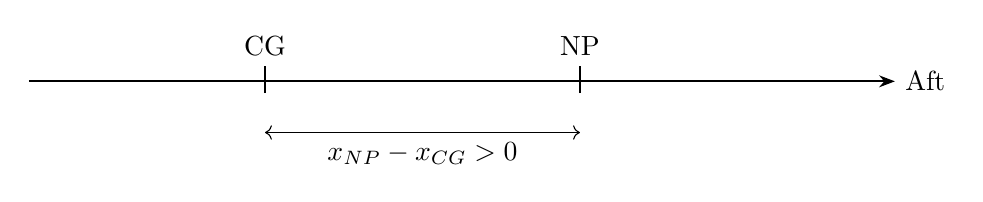
\begin{tikzpicture}[x=1cm,y=1cm]
\draw[arr] (0,0)--(11,0) node[right]{Aft};
\draw (3,-0.15)--(3,0.2) node[above]{CG};
\draw (7,-0.15)--(7,0.2) node[above]{NP};
\draw[<->] (3,-0.65)--node[below]{$x_{NP}-x_{CG}>0$}(7,-0.65);
\end{tikzpicture}
\end{center}
\begin{itemize}
\item \textbf{$SM>0$: CG ahead of NP.} If $\alpha$ increases, the aircraft gets a nose-down moment that pushes it back. This means it is statically stable.
\item \textbf{$SM=0$: CG at NP.} There is no restoring moment from a small change in $\alpha$, so the aircraft is neutrally stable in the static sense.
\item \textbf{$SM<0$: CG behind NP.} If $\alpha$ increases, the aircraft gets a nose-up moment that makes the disturbance larger. It is statically unstable unless a stability system corrects it.
\end{itemize}
For example, if the NP is at $40\%$ MAC and the CG is at $30\%$ MAC, then $SM=0.10$, or $10\%$ MAC. Moving the CG closer to the NP makes the aircraft less stable, but it usually takes less control effort to manoeuvre. A larger positive margin gives a stronger restoring effect, though it may also take more effort to trim and control.

The NP can change with the aircraft configuration and with whether the elevator is fixed or free, so the same condition should be used when finding the static margin. A positive margin means the aircraft has a restoring tendency; it does not tell us how quickly an oscillation dies out.

\newpage
\section*{Question 2}
Describe the differences between MCAS (Maneuvering Characteristic Augmentation System) and SAS (Stability Augmentation System) of longitudinal motion.

\textbf{Solution}

MCAS and a longitudinal SAS both affect pitch, but they do different jobs.

\textbf{MCAS} is used on the Boeing 737 MAX to reduce its pitch-up tendency at high angle of attack and make the handling feel as intended. It can operate in manual flight, with the flaps up and angle of attack high, and commands nose-down stabilizer trim.

\textbf{SAS} is used to improve stability and damping. For example, a pitch-rate gyro can detect unwanted pitching, and the SAS moves the elevator or tailplane to oppose that motion. This helps the aircraft settle down after a disturbance.

The main differences are:
\begin{enumerate}
\item \textbf{Purpose:} MCAS changes handling at high angle of attack. SAS improves stability and reduces unwanted motion.
\item \textbf{Input:} MCAS uses angle of attack and other flight-condition information. A basic longitudinal SAS uses pitch rate $q$, while a more advanced one may also use angle of attack or normal acceleration.
\item \textbf{Output:} MCAS commands nose-down stabilizer trim when its conditions are met. SAS moves the elevator or tailplane to oppose the disturbance.
\item \textbf{Operation:} MCAS only works under certain conditions. SAS gives feedback while it is switched on and within its operating range. It can also be part of an autopilot.
\end{enumerate}
For a simple pitch damper, the stabilizing moment can be represented by
\[
M_{\mathrm{SAS}}=-K_q q,\qquad K_q>0,
\]
where nose-up moment and pitch rate are positive. When the aircraft pitches up, the SAS produces a nose-down moment. When it pitches down, the correction is in the opposite direction.

So, MCAS is a specific feature for changing handling, while SAS is a more general system for improving stability. MCAS is not an altitude-hold autopilot or a complete stall-prevention system.


The updated MCAS compares both angle-of-attack sensors and limits when and how much it can activate. Its basic purpose is still to change the handling.

\newpage
\section*{Question 3}
Explain what is triplex redundant system and compare the differences between quadruplex and triple redundant systems.

\textbf{Solution}

A \textbf{triple redundant (triplex) system} has three channels doing the same job. It compares their outputs and uses a majority vote to find a channel that disagrees. For example, if A and B give similar outputs but C is very different, C can be treated as faulty and disconnected. The other two channels keep working.

The diagram below shows the four parallel channels of a quadruplex system.

\begin{center}
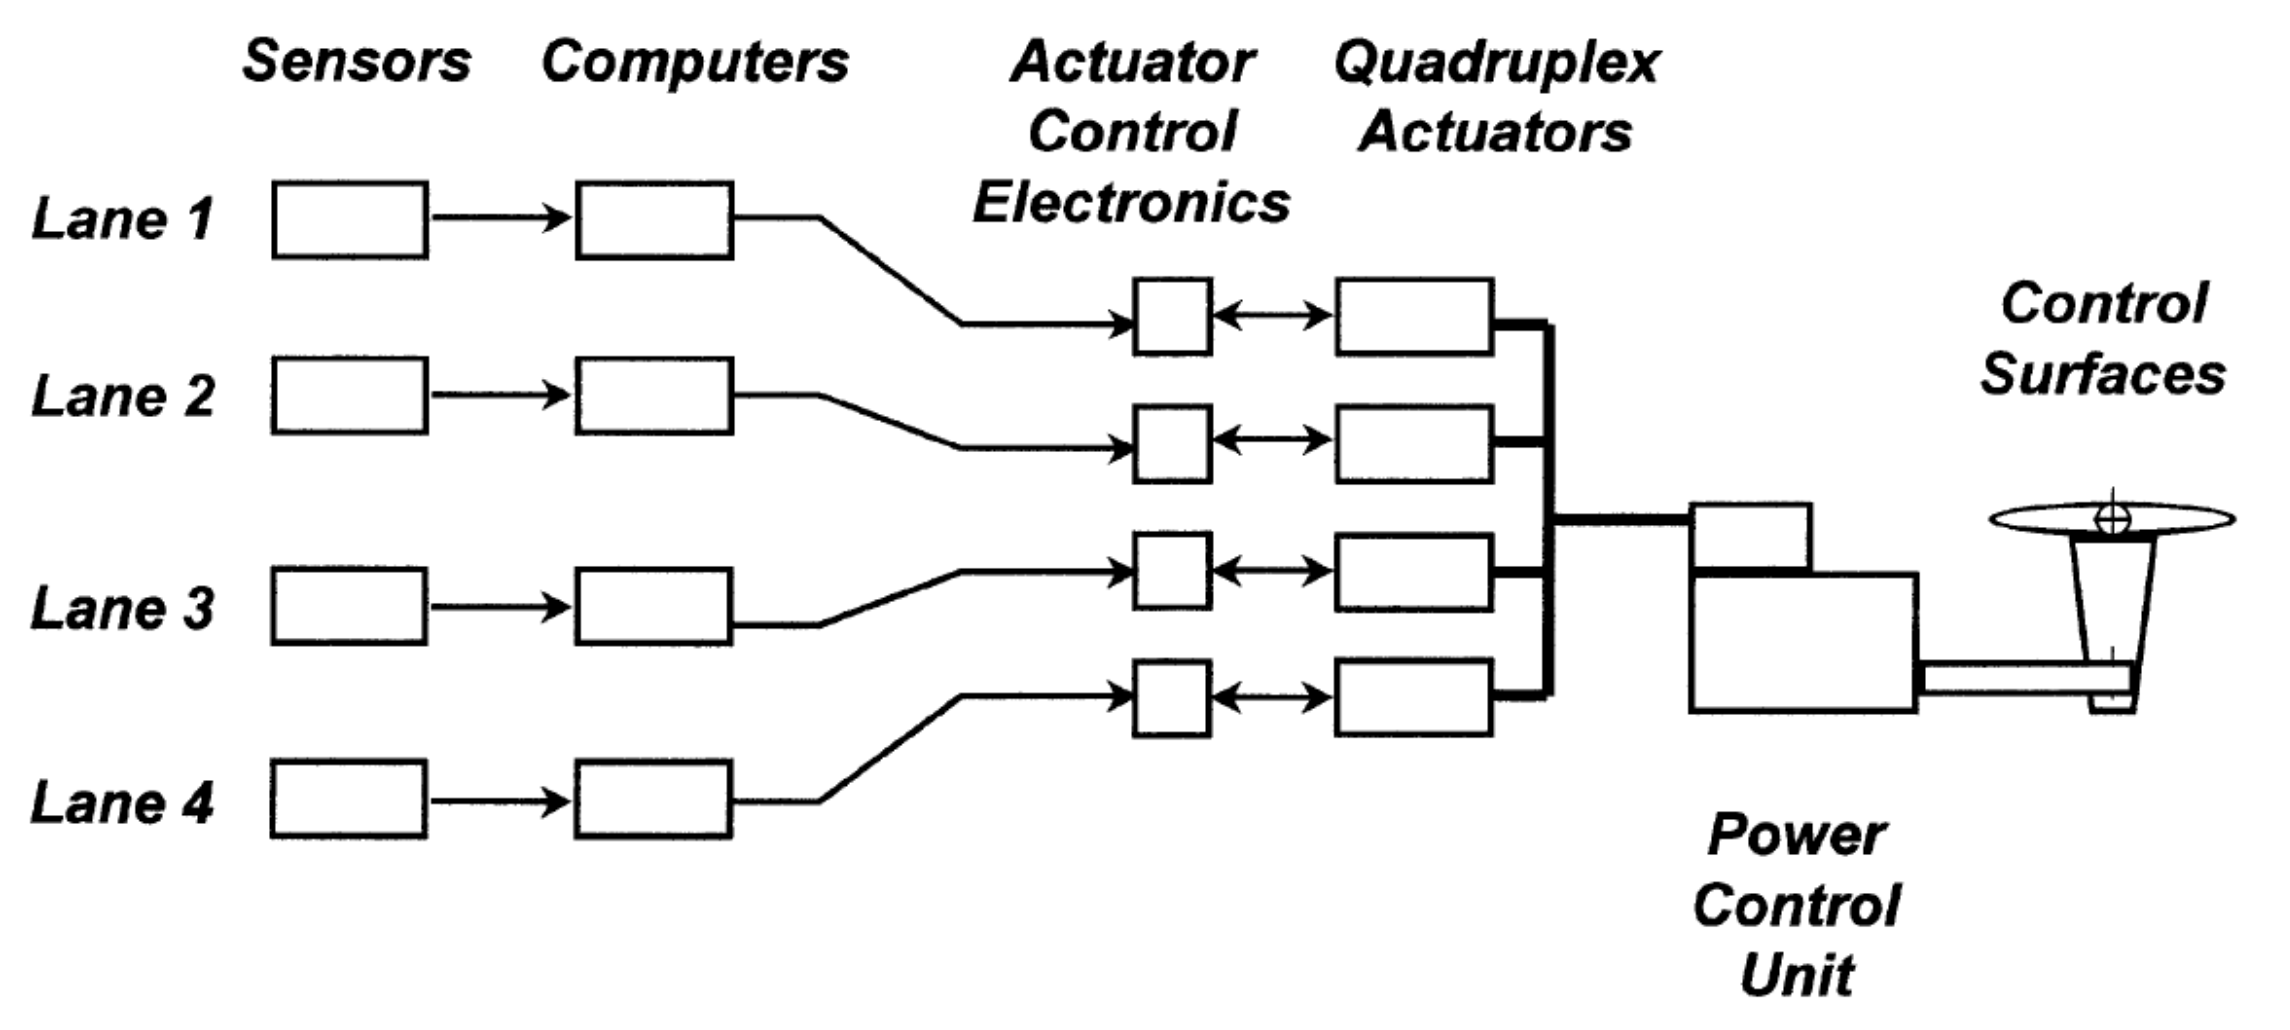
\includegraphics[width=11cm]{redundancy.png}
\end{center}

\small
\begin{tabular}{@{}P{3.0cm}P{5.9cm}P{6.2cm}@{}}
\toprule
Feature & Basic triplex & Quadruplex \\
\midrule
Channel count & Three. & Four. \\
\addlinespace
First independent failure & Two good channels agree, so the faulty one can be disconnected. Two channels remain. & Three good channels agree, so the faulty one can be disconnected. Three channels remain. \\
\addlinespace
Second sequential failure & Two remaining channels can disagree, but comparison alone cannot tell which is correct. & After the first faulty channel is removed, the remaining three can vote again. A second faulty channel can be removed, leaving two. \\
\addlinespace
Typical failure survival & One channel failure by majority voting. & Two separate failures, if each is detected and disconnected in time. \\
\addlinespace
Weight and cost & Less hardware, weight, power use, and cost. & More hardware, weight, and cost, but voting is still available after the first failure. \\
\bottomrule
\end{tabular}
\normalsize

A \textbf{monitored triplex} system works a little differently from basic voting. Each channel has its own monitor that can detect a failure. If the monitors work reliably, the system can disconnect two faulty channels and keep running on the one good channel.

For quadruplex to handle a second failure, the first faulty channel needs to be removed before the system is left with a two-against-two disagreement. It still cannot handle every pair of failures that happen at the same time. Both systems also need separate power, sensors, and actuators, because one shared failure could affect multiple channels.
\newpage
\section*{Question 4}
Please describe the advantages of radio navigation, dead reckoning, and fixed point positioning. Is it possible to use only one navigation system for the commercial airliners? Why?

\textbf{Solution}

These three methods give the aircraft different kinds of navigation information. In this answer, \textbf{fixed point positioning} means \textbf{position fixing}: finding the aircraft's position from outside references instead of just adding up its movement from an earlier position.

\begin{enumerate}
\item \textbf{Radio navigation:} Signals from known stations give bearing, range, or guidance. For example, VOR gives bearing information and DME gives slant range. Radio navigation works without seeing landmarks and can provide useful route and approach guidance. When signals are available, radio measurements can also correct INS position error. The drawbacks are limited coverage, poor station geometry, interference, or equipment outages.
\item \textbf{Dead reckoning (DR):} The aircraft updates its position from a known starting point using velocity and elapsed time. This gives continuous navigation between position fixes. An INS is self-contained and passive, so it can keep working if outside signals are lost. Air-data DR can also be a backup, but it needs an estimate of the wind. Its main drawback is that errors in starting position, speed, and heading build up over time.
\item \textbf{Position fixing:} The aircraft finds its position using outside references, such as GNSS satellites, intersecting radio measurements, or visible landmarks. A new fix can reduce errors that have built up during DR, so repeated fixes help limit long-term drift. However, accuracy and availability depend on signal quality and reference geometry; visual fixes also need good visibility.
\end{enumerate}

These categories can overlap. For example, VOR/DME radio navigation can also be used to get a position fix. Radio navigation describes the type of measurement, while DR and position fixing describe how the position is worked out.

\textbf{Using only one system:} One system might be enough for part of a flight, but using only one source for the whole flight would leave the aircraft with little backup. INS drifts, radio aids do not cover everywhere, and GNSS signals can be lost or corrupted. Even several copies of the same type of system can share the same failure.

Commercial aircraft therefore use several independent sources, preferably of different types. INS keeps navigation going between fixes, while GNSS or radio fixes help correct long-term errors. The systems can also be checked against one another, and the FMS can use the sources that are still available.

\newpage
\section*{Question 5}
What are the error sources of INS? How to reduce these errors?

\textbf{Solution}

An INS calculates velocity and position by integrating accelerometer measurements. This means small sensor or attitude errors can turn into large position errors over time.

\begin{enumerate}[itemsep=0.15em]
\item \textbf{Accelerometer errors:} Bias, scale-factor error, noise, or misalignment can make the measured acceleration wrong. For a constant bias $b_a$, a simple short-time model gives
\[
\delta v=b_a t,\qquad \delta r=\tfrac12 b_a t^2.
\]
\item \textbf{Gyro errors:} Bias or drift, scale-factor error, and noise cause attitude errors. A small tilt error $\delta\theta$ makes some gravity appear in a horizontal channel, creating an acceleration error of about $g\delta\theta$. If a constant gyro bias $b_g$ causes $\delta\theta\approx b_g t$, then at first
\[
|\delta r|\approx\tfrac16 g|b_g|t^3,
\]
where $b_g$ is in rad/s. Heading errors also resolve velocity along the wrong direction.
\item \textbf{Initial-condition errors:} If the starting position, velocity, levelling, or heading is wrong, the INS solution starts off wrong too.
\item \textbf{Environment and computation:} Temperature changes, vibration, ageing sensors, timing errors, and imperfect gravity or Earth models all add error. Incorrect Earth-rate, transport-rate, or Coriolis corrections also affect the result. Strapdown systems need good coning and sculling corrections when the aircraft is rotating and accelerating at the same time.
\end{enumerate}

\textbf{Ways to reduce the errors:}
\begin{itemize}[itemsep=0.15em]
\item Use accurate gyros and accelerometers; calibrate bias, scale factor, and alignment, and apply temperature compensation and suitable vibration isolation.
\item Start with a reliable position and velocity, and complete accurate levelling and heading alignment before navigation.
\item Use correct Earth/gravity models, synchronized measurements, sufficient sampling rates, and appropriate numerical and coning/sculling algorithms.
\item Aid the INS with independent GNSS or radio position fixes and, where available, velocity measurements. A Kalman filter can estimate navigation errors and observable sensor biases. Barometric altitude helps stabilize the vertical channel.
\end{itemize}

The $t^2$ and $t^3$ equations are only short-time approximations. In a local-level INS, Schuler tuning affects how horizontal errors change, with a period of about 84.4 minutes. It helps control tilt-related errors, but does not remove all drift, so the INS still needs outside updates for long-term accuracy.

\newpage
\section*{Question 6}
Please show the differences between the strapdown and stable gimbal systems.

\textbf{Solution}

Both systems use gyros and accelerometers to find attitude, velocity, and position. The main difference is how they keep track of the reference axes: with a moving platform or with calculations.

\begin{center}
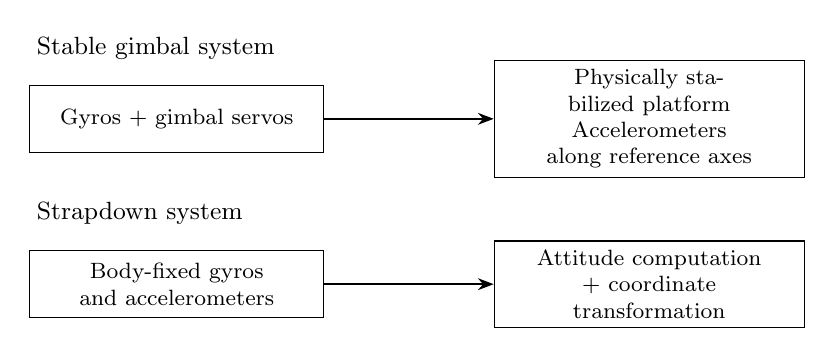
\begin{tikzpicture}[x=1cm,y=1cm]
\node[block,text width=3.5cm] (g1) at (0,0) {Gyros + gimbal servos};
\node[block,text width=3.7cm] (g2) at (6,0) {Physically stabilized platform\\Accelerometers along reference axes};
\draw[arr] (g1)--(g2);
\node[font=\small,anchor=west] at (-1.9,0.9) {Stable gimbal system};
\node[block,text width=3.5cm] (s1) at (0,-2.1) {Body-fixed gyros\\and accelerometers};
\node[block,text width=3.7cm] (s2) at (6,-2.1) {Attitude computation\\+ coordinate transformation};
\draw[arr] (s1)--(s2);
\node[font=\small,anchor=west] at (-1.9,-1.2) {Strapdown system};
\end{tikzpicture}
\end{center}

\small
\begin{tabular}{@{}P{2.5cm}P{6.0cm}P{6.6cm}@{}}
\toprule
Feature & Stable gimbal (platform) & Strapdown \\
\midrule
Mounting & Sensors are mounted on a platform inside gimbals. & Sensors are rigidly attached to the aircraft. \\
\addlinespace
Reference axes & Gyros and servos keep the platform aligned with the chosen navigation frame. & A computer maintains a virtual reference frame from gyro measurements. \\
\addlinespace
Measurements & Accelerometers measure along platform axes; gimbal pick-offs provide attitude angles. & Sensors measure body-axis specific force and angular rate; attitude and navigation-axis forces are computed. \\
\addlinespace
Hardware & Gimbals, bearings, motors, and pick-offs add size, weight, and maintenance. & Fewer moving mechanical parts allow a compact, robust installation. \\
\addlinespace
Computation & Less high-rate attitude transformation is required, but navigation corrections are still needed. & Requires fast attitude updates, coordinate transformations, and coning/sculling compensation. \\
\addlinespace
Limitations & Gimbal travel limits, friction, servo errors, and possible mechanical gimbal lock. & Sensors must handle full body motion; sampling and algorithm errors matter. \\
\bottomrule
\end{tabular}
\normalsize

In a strapdown system, $\mathbf f^n=C_b^n\mathbf f^b$. Here, $C_b^n$ changes the measured body-axis specific force into navigation axes. The system then applies gravity and rotation corrections before integration. A gimballed system gets the same reference by physically keeping the platform aligned.

Using quaternions in a strapdown system avoids a mathematical problem that can happen when propagating attitude with Euler angles. Accuracy still depends on the sensors, calibration, alignment, and calculations. Both types need gravity and Earth-rate corrections, and both can use Schuler tuning and outside updates.

\newpage
\section*{Question 7}
What is the fundamental concept of the dead reckoning DR navigation? Use a diagram and some equations to show the process of DR navigation.

\textbf{Solution}

Dead reckoning continuously estimates where the aircraft is by adding up how far it has travelled from a known starting point. It integrates \textbf{ground velocity}, rather than using airspeed alone:
\[
\boxed{\mathbf r(t)=\mathbf r_0+\int_{t_0}^{t}\mathbf V_g(\tau)\,d\tau.}
\]
The vector equation uses a local frame where the Earth is treated as approximately flat. For air-data DR, ground velocity comes from adding the horizontal air-velocity and wind vectors.

\begin{center}
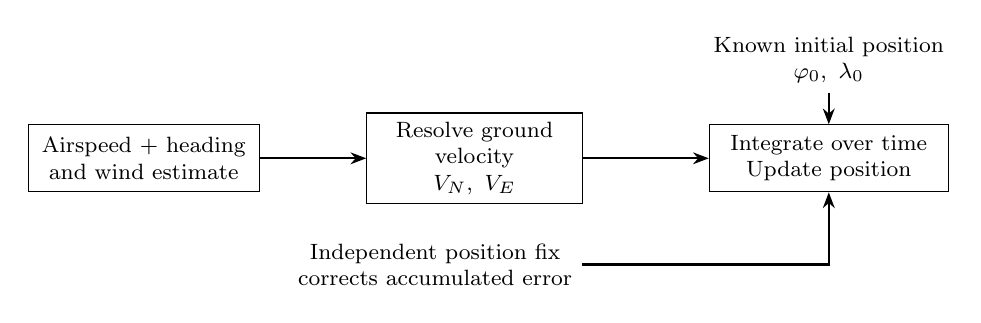
\begin{tikzpicture}[x=1cm,y=1cm]
\node[block,text width=2.7cm] (a) at (0,0) {Airspeed + heading\\and wind estimate};
\node[block,text width=2.5cm] (v) at (4.2,0) {Resolve ground velocity\\$V_N,\ V_E$};
\node[block,text width=2.8cm] (p) at (8.7,0) {Integrate over time\\Update position};
\draw[arr] (a)--(v);
\draw[arr] (v)--(p);
\node[font=\footnotesize,align=center] (init) at (8.7,1.25) {Known initial position\\$\varphi_0,\ \lambda_0$};
\draw[arr] (init)--(p);
\node[font=\footnotesize,align=center] (fix) at (3.7,-1.35) {Independent position fix\\corrects accumulated error};
\draw[arr] (fix.east)-|(p.south);
\end{tikzpicture}
\end{center}

Let $\psi$ be the true heading measured clockwise from north, and let $V_h$ be horizontal airspeed. Assume sideslip is small. If $W_N,W_E$ are the north and east wind components, measured in the direction the wind is moving, then
\[
V_N=V_h\cos\psi+W_N,\qquad
V_E=V_h\sin\psi+W_E.
\]
For approximately level flight, $V_h\approx V_{\mathrm{TAS}}$. Ground speed and true track $\chi$ are
\[
V_g=\sqrt{V_N^2+V_E^2},\qquad
\chi=\operatorname{atan2}(V_E,V_N).
\]
Using a spherical Earth of radius $R$ at altitude $h$, latitude $\varphi$ and longitude $\lambda$ are updated in radians by
\[
\boxed{\begin{aligned}
\varphi_{k+1}&=\varphi_k+\frac{V_{N,k}\Delta t}{R+h},\\
\lambda_{k+1}&=\lambda_k+\frac{V_{E,k}\Delta t}{(R+h)\cos\varphi_k}.
\end{aligned}}
\]
These step-by-step equations assume velocity stays almost constant during each short time interval. This latitude/longitude method does not work well near the poles.

For example, if the aircraft flies north at 120 kt TAS and the wind blows east at 20 kt, then $V_N=120$ kt and $V_E=20$ kt. After 30 minutes, it has travelled about 60 NM north and 10 NM east. This shows why track and heading are not always the same.

Errors in the starting fix, heading, airspeed, wind, or timing build up as the aircraft travels. Independent position fixes can correct the estimate from time to time. Doppler DR measures ground velocity directly, while INS works it out from acceleration, but both follow the same idea of integrating displacement.

\end{document}
